\begin{figure}
\begin{center}
    \centering
    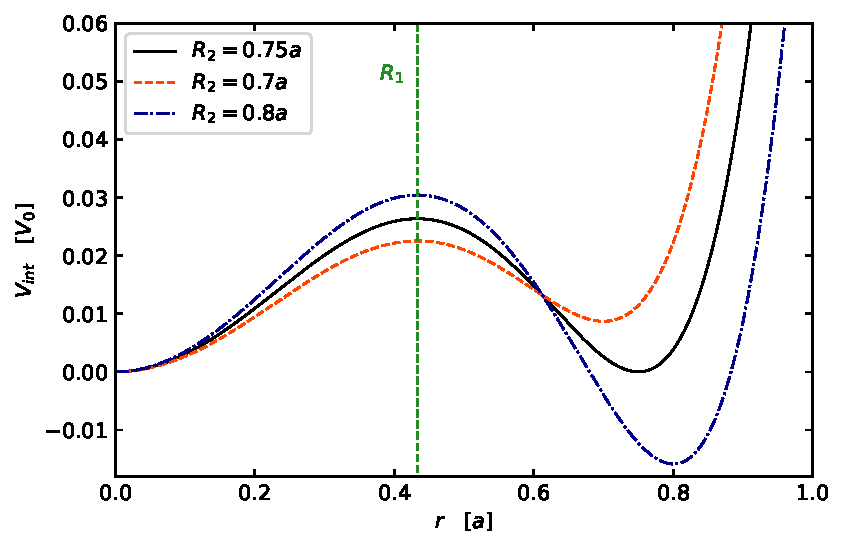
\includegraphics[width=1\linewidth]{Images/V_int.pdf}
    \caption{The molecular potential $V_\text{int}$ of Eq.~\eqref{eq:V_int} for fixed amplitude $U = 1 \p$ and location of the local maximum $R_1 = \frac{\sqrt{3}}{4} a$, and three different values of $R_2$. The first minimum is at the origin with null energy, the maximum is at $R_1$ and the second minimum at $R_2$.}
    \label{Fig:V_int}
\end{center}
\end{figure}

\begin{table}[]
    \centering
    \renewcommand\arraystretch{1.4}
    \begin{tabular}{c|c}
        \toprule
        Physical quantities &  Model units\\
        \midrule
        length             &   $a$   \\
        mass               &   $m$   \\
        energy             &   $V_0$  \\
        time               &   $\tim$   \\
        frequency and viscosity $\gamma$           &   $\freq$ \\
        force              &   $\f$    \\
        velocity           &   $\vel$  \\
        potential prefactor $U$        &   $\p$  \\
        \bottomrule
    \end{tabular}
    \renewcommand\arraystretch{1.2}
    \caption{All the relevant physical quantities for our work with their corresponding natural units}
    \label{tab:natural_units}
\end{table}


For the external corrugated potential $V_\text{ext}$ where the particles move we adopt the simplest periodic function:
\begin{equation}
    V_\text{ext}(x) = - \frac{V_0}{2}\cos\left(\frac{2\pi}{a}x \right), 
\end{equation}
where $V_0$ is the peak-to-peak energy amplitude, and $a$ is the period of the potential. We adopt the energy $V_0$, the length $a$ and the mass $m$ of each particle in the molecule as basic units, obtaining a system of natural units for the model, summarized in Table~\ref{tab:natural_units}. \\

The molecule is represented by two identical point-like particles of mass $m$ bounded together by a molecular bistable potential $V_\text{int}$ depending only on the distance between the particles. %The internal motion is so a one-dimensional problem, with only one degree of freedom.
The adopted analytical form of the potential has a first stable minimum at the origin at null energy, and a second minimum separated to the first by a barrier. The explicit expression is:
\begin{equation}
    V_\text{int}(r) = f( \zeta = r^2) = U\left[\zeta^3- \frac{3}{2}(R_1^2 + R_2^2)\zeta^2 + 3 R_1^2 R_2^2 \zeta \right],
    \label{eq:V_int}
\end{equation}
where $r = |x_2 - x_1|$ is the distance between the two particles, $U$ is a parameter that scales the strength of the potential, and $R_1$ and $R_2$ are the positions of the barrier and of the second stable minimum respectively, as sketched in Fig.~\ref{Fig:V_int}. Given that $R_1$ and $R_2$ have the dimension of a length, and so does $r$, $U$ must be an energy divided by a length to the sixth power. In general, the second minimum can be lower or higher in energy than the one at the origin, but if we select $R_2 = \sqrt{3}R_1$, it is at the same (zero) energy as the first minimum. Regardless of the fact that the minimum at $R_2$ can be either a local or an absolute minimum, in this work we will always refer to the potential barrier $\delta = V_\text{int}(R_1) - V_\text{int}(R_2)$. $\delta$ is the barrier that the molecule has to overcome to jump from the minimum at $R_2$ to the one at the origin. This definition is meaningful even when the origin is a local minimum and $R_2$ the absolute minimum because, practically, at null temperature and for equal drag coefficients on the two atoms, once the molecule is at zero, it has no chances of escaping to $R_2$. While the passage from zero to $R_2$ is not possible, the opposite usually is, and it may be fastened by the interaction of the molecule with $V_\text{ext}$. If $R_2 > \sqrt{3}R_1$, then $V_\text{int}(R_2) > 0$, and therefore the barrier $\delta$ is smaller than $V_\text{int}(R_1)$. On the contrary, if $R_2 < \sqrt{3}R_1$, then $V_\text{int}(R_2) < 0$ and $\delta > V_\text{int}(R_1)$. This can be easily verified by looking at the explicit expressions of $V_\text{int}(R_1)$, $V_\text{int}(R_2)$ and their difference:
\begin{align}
    \notag
    \delta = V_\text{int}(R_1) - V_\text{int}(R_2) = U\frac{R_2^6}{2}\left[ 3\left(\frac{R_1}{R_2}\right)^4 -  \left(\frac{R_1}{R_2}\right)^6 \right]
    -U\frac{R_2^6}{2}\left[ 3\left(\frac{R_1}{R_2}\right)^2 - 1\right] = \\
     = U\frac{R_2^6}{2}\left[ 1 -  \left(\frac{R_1}{R_2}\right)^6 + 3\left(\frac{R_1}{R_2}\right)^4  - 3\left(\frac{R_1}{R_2}\right)^2 \right].
    \label{eq:delta}
\end{align}
As can be seen, the magnitude of the potential barrier scales rapidly as $UR_2^6$\\


We shall now proceed to write the equations of motion. Starting from the full Hamiltonian of the system
\begin{equation}
    H = \sum_{i=1}^2 \left( \frac{p_{i}^2}{2m} + V_\text{ext}(x_i) - Fx_i \right) + V_\text{int}(|x_2 - x_1|),
\end{equation}
we obtain the classical Newton's law for the motion of the two particles:

\begin{align} 
    m \ddot{x}_{1}=F-\frac{V_{0} \pi}{a} \sin \left(\frac{2 \pi}{a} x_{1}\right)+ V'_\text{int}(r)-m \gamma \dot{x}_{1} \label{eq:x1},\\
    m \ddot{x}_{2}=F-\frac{V_{0} \pi}{a} \sin \left(\frac{2 \pi}{a} x_{2}\right)- V'_\text{int}(r)-m \gamma \dot{x}_{2}
    \label{eq:x2},
\end{align}
where 
\begin{equation}
    V'_\text{int}(r) = U\left[6\left(x_{2}-x_{1}\right)^{5}-6\left(x_{2}-x_{1}\right)^{3}\left(R_{1}^{2}+R_{2}^{2}\right)+6\left(x_{2}-x_{1}\right) R_{1}^{2} R_{2}^{2}\right],
\end{equation}
$F$ is the constant external force that we apply to the two particles. The dissipative term $m\gamma \dot{x}_{i}$ is non-Hamiltonian in nature, and must be adopted to dissipate the energy pumped in the system by the constant external force, and prevents states with constantly growing velocity. Thanks to this damping term we can obtain states with regular advancement, that are precisely what we plan to investigate. Physically, the $\gamma$ term accounts for the viscous friction that a real molecule is subject to when moving in a fluid.

The system is described by two coupled nonlinear ordinary differential equations (ODE), Eq.~\eqref{eq:x1} and~\eqref{eq:x2}. As we cannot see any exact analytical solution, we integrate these equations numerically by means of a Runge-Kutta-Fehlberg method, as descried in App.~\ref{appendix:sec}. The algorithm is capable of adjusting automatically the integration time step to maintain a prescribed accuracy~\cite{RKF45,RKF45_b}. Our code requires the specification of the following dynamical parameters of the model:
$R_1$, $R_2$, $U$, $F$, $\gamma$.
In addition, we need to set the initial conditions. We will call $R_0$ the initial value of $r =|x_2 - x_1|$. If not specified, the first particle is placed at the origin ($x_1=0, x_2 = R_0$), and both initial velocities are zero. 
